			One of the main challenges of empirical economics is identifying causal effects. Identifications strategies such as Regression Discontinuity (RD), Instrumental Variables (IV), Difference-in-Differences (DiD) and event studies help us achieve this goal. To do so, these strategies only use part of the variation in the data. They exploit the exogenous part of the variation in the treatment or decrease the sample size by only considering observations for which the as-if random assignment assumption is credible. This reduction in the variation used can decrease precision and thus statistical power---the probability of rejecting the null hypothesis when it is false, or put simply, the probability of obtaining a statistically significant estimate. There is therefore a tension between reducing confounding and statistical power.
			
			When statistical power is low, not only is the estimator imprecise but statistically significant estimates exaggerate the true effect size \citep{ioannidis_why_2008, gelman_beyond_2014, lu_note_2019, zwet_significance_2021}. Only estimates at least 1.96 standard errors away from zero are statistically significant at the 5\% level. In under-powered studies, these estimates make up a selected sub-sample of all estimates, located in the tails of the distribution of all possible estimates. The average of these statistically significant estimates differs from the true effect, located at the center of the distribution if the estimator is unbiased. In addition, the less precise the estimator, the larger exaggeration is.  \Cref{fig:graph_exag} illustrates the inflation of significant estimates caused by imprecision. When power is low, obtaining a statistically significant estimate from an unbiased estimator does not guarantee that it will be close to the true effect. An estimator $\hat{\beta}$ of the true effect $\beta$ might be unbiased in the traditional sense of $\mathbb{E}[\hat{\beta}] = \beta$ but conditionally biased in the sense that $\mathbb{E}[\hat{\beta} | \text{ Significant}] \neq \beta$. For statistically significant estimates, the tension between statistical power and reducing confounding is thus a tension between reducing confounding and exaggerating the true effect size.
			
			   \begin{figure}[!h]
				\begin{center}
					\caption{Significance and distribution of two unbiased estimators with different variances}
					\label{fig:graph_exag}
					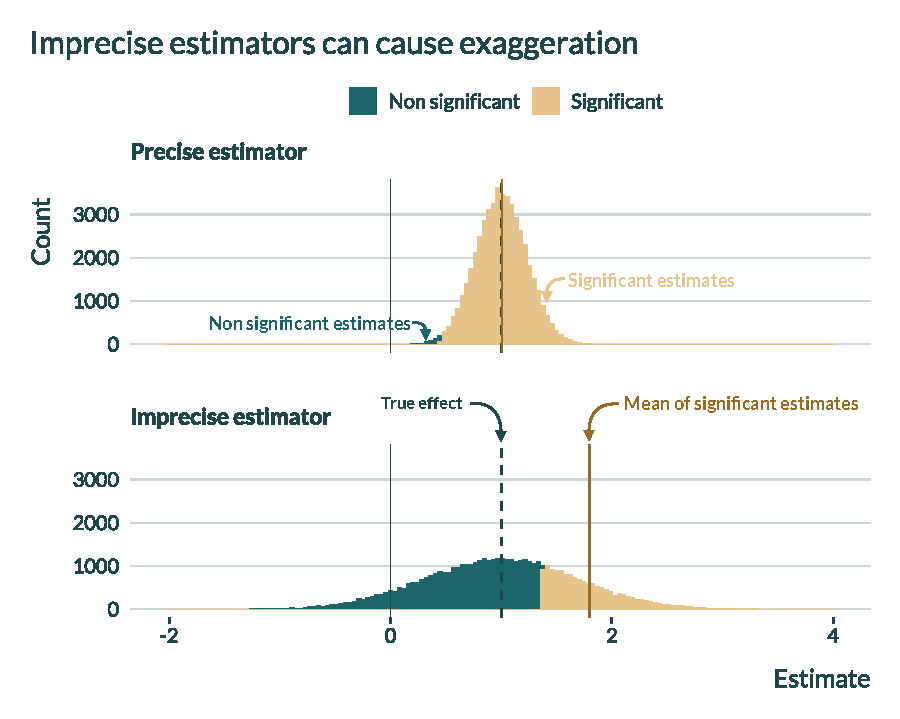
\includegraphics[width=0.8\linewidth]{images/graph_intuition_precision.pdf}
					\caption*{\footnotesize \textit{Notes}: 100,000 draws from two normal distributions $\mathcal{N}(1, 0.05)$ and $\mathcal{N}(1, 0.5)$.}
				\end{center}
				\vspace{-1cm}
			 \end{figure}
			
			Yet, exaggeration only arises when two circumstances are combined: 1) a publication bias favors statistically significant results and 2) statistical power is low. A large literature underlined the existence of the former in economics \citep[for instance]{rosenthal_file_1979, andrews_identification_2019, abadie_statistical_2020, brodeur_methods_2020}. Published estimates from under-powered studies thus form a biased sample of the distribution of estimates and can greatly exaggerate true effect sizes. Then, the economics literature, as others, suffers from a frequent and substantial lack of statistical power \citep{ioannidis_power_2017, ferraro_featureis_2020}. The resulting exaggeration has been documented as partly explaining the current replication failures observed in various fields such as economics, epidemiology, medicine or psychology \citep{button_power_2013, open_science_collaboration_estimating_2015, camerer_evaluating_2016, chang_is_2022}. Even in experimental economics, with a high level of control and an arguable absence of confounders, estimates published in top economic journals that have been replicated were on average inflated by a factor of at least 1.5 \citep{camerer_evaluating_2016}. Quasi-experimental studies are likely even more exposed to this exaggeration issue as, in current practices, statistical power is not central to such analyses. Several meta-analyses provide clear evidence of consequential exaggeration in the non-experimental economics literature. \cite{ioannidis_power_2017} finds that the median statistical power in a wide range of areas of economics is no more than 18\%. Despite the widespread use of convincing causal identification strategies and usually large sample sizes, they show that nearly 80\% of estimates are likely exaggerated by a factor of two. In environmental economics, \cite{ferraro_featureis_2020} finds that 56\% of estimates are exaggerated by a factor of two or more. In a companion paper, I document evidence of substantial exaggeration in a subfield of this literature, that on the acute health effects of air pollution \citep{bagilet_accurately_2023}. The magnitude of exaggeration is thus considerable and could in some situations be on par with that of a bias caused by confounders. 
			%Add CBA thing here
			It is thus crucial to take exaggeration into account and to understand its drivers.
			%In environmental economics, where estimates are often directly used to inform policies, in particular via CBA, obtaining accurate estimates is even more crucial. In this field, we often chase small and diffuse effects, that are intrinsically difficult to capture, often because playing a role in the long term or being causaly diffuse. 
			%It is even more important in some fields such as environmental economics where estimates are used to directly inform public policy. Via CBA 
			
			% goal of this study
			In this paper, I argue that the use of causal identification strategies contributes to exaggeration. %I propose an overarching mechanism that may contribute to do so. 
			Using a mathematical derivation and Monte Carlo simulations, I show that design choices in quasi-experimental studies can be seen as a trade-off between avoiding confounding and overestimating true effect sizes due to a resulting loss in power. To limit the threat of confounding, causal inference methods discard variation and therefore reduce statistical power. When combined with a statistical significance filter, this results in exaggeration bias. While causal identification strategies are essential to describe causal relationships, this paper emphasizes that a perfectly convincing identification does not guaranty an absence of ``bias'' and that improving identification can actually pull us away from the true effect. The same strategies which remove the bias caused by confounding factors actually introduce another type of bias.
			
			%mechanisms
			%I analyze the key factors affecting the confounding-exaggeration trade-off for a wide range of identification strategies : RD, IV, event studies, strategies such as DiD relying on  fixed effects (FEs) or generic controls and matching. 
			
			%IMPORTAAAAAANNNNTTT
			%Maybe change order
			All causal identification strategies discard variation in order to identify causal effects but the confounding-exaggeration trade-off is mediated through a distinctive channel for each of them. In RD designs, even when the initial sample size is large, we discard part of the variation by only considering observations within the bandwidth, decreasing the effective sample size and thus precision. In an IV setting, we only use the subset of the variation in the treatment that is explained by the instrument. In studies leveraging exogenous shocks, the variation used to identify an effect sometimes only comes from a limited number of changes in treatment status. Approaches that do not actually leverage natural experiments but aim to identify a causal effect by controlling for confounders also limit the variation used. 
			%When all confounders are arguably measured, matching has a causal interpretation but it still 
			Matching prunes units that cannot be matched and thus reduces the effective sample size. Adding controls or fixed effects to the model can increase the variance of the estimator and exaggeration if they absorb more of the variation in the treatment than in the outcome variable. 
			
			%IMPORTAAAAAANNNNTTT
			%I need to change and strengthen that: reorganize with the right id strats
			Since causal identification strategies can be interpreted as ways of controlling for confounders, this last point actually ties all the strategy-specific arguments together. We implement Fixed Effects (FEs) based identification strategies such as DiD to control for the invariant, unobserved, and arguably endogenous part of the variation in the outcome. In the Control Function (CF) approach to IV, we control for the variation in $x$ unexplained by the instruments. %the predicted residuals of the regression of the endogenous variable of interest on the instrument.
			 Fuzzy-RD and propensity score matching can also be thought of as control function approaches, of the forcing variable and propensity score respectively. In addition, excluding observations that are outside the bandwidth or unmatched is equivalent to controlling for observation-level fixed effects for these observations. When these methods for controlling for confounders absorb more of the variation in the treatment than in the outcome, they will increase the variance and cause exaggeration. Considering a simple linear homoskedastic model gives the intuition for this trade-off between exaggeration and omitted variable bias (OVB) for control approaches.  Let $y_{i} = \alpha + \beta x_{i} + \delta w_{i} + u_{i}$, $\forall i \in \{1, .., n\}$,  with $x$ the variable of interest, $w$ a potentially unobserved variable correlated with $x$ and $u$ an error term. Under usual assumptions and using the Frisch-Waugh-Lovell theorem, we get that $ \sigma_{\textsc{ovb}}^2$ and $ \sigma_{\textsc{ctrl}}^2$, the variance of the estimators for $\beta$ when omitting $w$ (short regression) and controlling for it (long regression) are respectively:
			~
			\[
				\sigma_{\textsc{ovb}}^2 =
				 \dfrac{\sigma^{2}_{u_{\textsc{ovb}}}}{n \ \sigma_{x}^{2}} =
				 \dfrac{\sigma^{2}_{y^{\perp x}}}{n \ \sigma_{x}^{2}}
				 \qquad \text{and} \qquad
				 \sigma_{\textsc{ctrl}}^2 = 
				 \dfrac{\sigma^{2}_{u_{\textsc{ctrl}}}}{n \ \sigma_{x^{\perp w}}^{2}} =
				  \dfrac{\sigma^{2}_{y^{\perp x, w}}}{n \ \sigma_{x^{\perp w}}^{2}}
			\]
			
			where $\sigma^{2}_{u_{\textsc{ovb}}}$ and $\sigma^{2}_{u_{\textsc{ctrl}}}$ are the variances of the residuals in the regression of $y$ on $x$ and of $y$ on $x$ and $w$ respectively, $\sigma^{2}_{y^{\perp x}}$ and $\sigma^{2}_{y^{\perp x, w}}$ are the variances of the parts of $y$ that are orthogonal to $x$ and to $x$ and $w$ respectively, $\sigma^{2}_{x}$ is the variance of $x$ and $\sigma^{2}_{x^{\perp w}}$ is the variance of the part of $x$ orthogonal to $w$. Thus,
			
			\[
				 \sigma_{\textsc{ctrl}}^2 > \sigma_{\textsc{ovb}}^2
				 	\quad \Leftrightarrow \quad 
				 	\dfrac{\sigma^{2}_{y^{\perp x, w}}}{n \ \sigma_{x^{\perp w}}^{2}} >
					\dfrac{\sigma^{2}_{y^{\perp x}}}{n \ \sigma_{x}^{2}} 
					\quad \Leftrightarrow \quad 
					\dfrac{\sigma^{2}_{y^{\perp x, w}}}{ \sigma_{y^{\perp x}}^{2}} >
					\dfrac{\sigma^{2}_{x^{\perp w}}}{\sigma_{x}^{2}}
			\]
			
			Controlling for $w$ will increase the variance of the estimator if the fraction of the variance unexplained by $w$ is greater for $y^{\perp x}$ than for $x$. Put differently, if controlling absorbs more of the variation in $x$ than in the residual part of $y$ ($y^{\perp x}$), it will increase the variance of the estimator. As briefly discussed above, since exaggeration increases with the variance of the estimator, controlling may increase exaggeration. I develop a formal proof showing that exaggeration can be larger when controlling, even when accounting for bias, in section \ref{maths}.
			
			% what we actually do
			In the remainder of the paper, I first derive a formal proof of the existence of the trade-off for prevailing causal identification strategies. Specifically, I show that the bias caused by exaggeration can be larger than the one caused by confounders. I also analyze the drivers of exaggeration and show that it increases as the strength of the instruments decreases, the number of exogenous shocks decreases or when controlling for a confounder absorbs more of the variation in the treatment than in the outcome. 
			
			 Then, I illustrate the existence of this ``causal exaggeration'' in realistic settings using examples drawn from environmental, education, labor, health and political economics. %We show that an actual trade-off between exaggeration and confounders can exist as exaggeration can be large for research designs implemented in actual studies. 
			The exaggeration of statistically significant estimates can be defined as the ratio of the estimated effect over the true effect, which is never known in a real world setting. I order to know the true effect and be able to compute this quantity, I turn to simulations. In addition, Monte-Carlo simulations allow to vary the value of the parameter of interest \textit{ceteris paribus}. An actual setting would for instance only allow to observe one strength for a given instrument. Since these simulations have an illustrative purpose only, I intentionally focus on settings in which statistical power can be low. All other simulation assumptions are chosen to make it as easy as possible to recover the effect of interest. I consider simple linear models with constant and homogenous treatment effects, \textit{i.i.d.} observations and homoskedastic errors. All the models are correctly specified and accurately represent the data generating process, except for the omitted variable.
									
			Finally, I discuss concrete avenues to address this causal exaggeration when carrying out a non-experimental study\footnote{In experimental studies, a solution to increase power is generally to increase sample size, reduce noise by improving measurement or improving balance or focus on larger potential effects.}. First, I advocate for the use of tools to evaluate the potential magnitude and risk of both confounding and exaggeration issues separately. Sensitivity analyses help with the former while power calculations help with the latter. %These power calculations can be computed before and after the analysis is carried out. 
			For instance, the sensitivity analysis tools developed in \cite{cinelli_making_2020} enable to assess how strong confounders would have to be to change the estimate of the treatment effect beyond a given level we are interested in. Then, considering the attention given to bias avoidance in the economics literature, I advocate to make power central to non-experimental analyses, even after an effect has been found, in order to limit bias caused by exaggeration. Prospective power simulations help identify the design parameters affecting power and exaggeration by approximating the data generating process \citep{gelman_regression_2020, black_simulated_2021}. Retrospective power calculations allow to evaluate whether a study would have enough power to confidently estimate a range of smaller but credible effect sizes \citep{gelman_beyond_2014, stommes_reliability_2021}.
			%%%%%%%% Evaluating potential exaggeration and confounders is however complex as both rely on unobserved shit
			Focusing more specifically on the trade-off and its drivers, I present tools to visualize the variation actually used for identification when using causal identification strategies. The \href{https://vincentbagilet.github.io/causal_exaggeration/}{companion website} describes in details how such analyses can be implemented. Finally, I briefly discuss potential solutions to mitigate this trade-off.
						
			% first contribution
			This paper contributes to three strands of the applied economics literature. First, the idea that causal identification estimators, while unbiased, may be imprecise is not new; this is part of the well-known bias-variance trade-off \citep{imbens_optimal_2012, deaton_understanding_2018, hernan_causal_2020, ravallion_should_2020}. I approach this literature from a different angle: through the prism of statistical power and publication bias. Not only the limited precision resulting from the use of causal identification methods could make it difficult to draw clear conclusions regarding the exact magnitude of the effect but I argue that it might also inherently lead to inflated published effect sizes, creating another ``bias''. The bias-variance trade-off can in fact be a bias-bias trade-off.
			
			% second contribution
			Second, studies discussing the exaggeration of statistically significant estimates due to a lack of power usually do not investigate its determinants and focus on specific causal identification methods separately \citep{ioannidis_power_2017, schell_evaluating_2018, ferraro_featureis_2020, black_simulated_2021, stommes_reliability_2021, young_leverage_2021}.  In a companion paper, I highlight tangible design parameters that can cause exaggeration for a wide range of empirical designs \citep{bagilet_accurately_2023}. In the present paper, I take a step back and propose an overarching mechanism, inherent to causal identification strategies as a whole, and that can explain these issues: although each strategy does so through different means, in essence they discard part of the variation, thereby increasing the risks of exaggeration. %This connection could be exacerbated by the fact that, as noted by \cite{brodeur_methods_2020}, publication bias is more prevalent for some methods such as the IV. 
			
			% third contribution
			Third, this study contributes to the literature on replicability in economics \citep{camerer_evaluating_2016, ioannidis_power_2017, christensen_transparency_2018, kasy_forking_2021}. The trade-off presented in this paper suggests that the widespread use of convincing causal identification methods in economics may not shield the field from potential replication threats.
			%The trade-off presented in this paper may contribute to explaining the replication failures observed in empirical economics, despite the widespread use of convincing causal identification methods.
			
			In the following section, I study the drivers of exaggeration and formally show in a simple setting that the use of causal identification strategies can exacerbate it. In section  \ref{simulations}, I implement realistic Monte-Carlo simulations to illustrate the existence of the confounding-exaggeration trade-off. I discuss potential solutions to navigate this trade-off in section \ref{discussion} and conclude in section \ref{conclusion}.
	
	
		